\documentclass{article}
\usepackage[utf8]{inputenc}
\usepackage{amsmath,mathtools}
\usepackage{subfiles}
\usepackage[
    natbib=true,
    style=numeric-comp,
    sorting=none,
    url=false,
    isbn=false,
    eprint = false,
]{biblatex}
\addbibresource{My Library.bib}
\usepackage[colorlinks=true, allcolors=black]{hyperref}
\usepackage{cleveref}
\usepackage{todonotes}
\usepackage{physics}
\usepackage{siunitx}
\usepackage{bm}
\usepackage{caption}
\usepackage{subcaption}
\usepackage{appendix}
\usepackage{graphicx}
\usepackage{layout}
\usepackage{amsfonts} 
\usepackage{amsthm}
\usepackage[version=4]{mhchem}
\newtheorem{example}{Example}
\newtheorem{theorem}{Theorem}
\newtheorem{lemma}{Lemma}
\newtheorem{definition}{Definition}

\newcommand\Mach{\mbox{\textit{Ma}}}  % Reynolds number
\newcommand\Froude{\mbox{\textit{Fr}}}  % Froude number


\begin{document}
\section{Fundamentals of heat transfer correlations}
\textbf{TODO: force myself to make summary of KC}
\section{Heat conduction in insulation}
The radial heat conduction in the tank wall can be calculated by dividing the wall into thin concentric shells, and solving the heat equation using a finite volume method. The radial heat conduction is given by the equation
\begin{equation}
    \rho c_{p} \partial_{t} T\left( r,t \right)
    = \frac{1}{r}\partial_{r} \left( r \kappa \partial_{r} T\left( r,t \right)
    \right)
    \label{eq:heat_equation}
\end{equation}
Integrating over one cell gives
\begin{equation}
    \rho c_{p} \partial_{t} \Theta + \frac{f_{i-1/2} - f_{i+1/2}}{2 \pi r_{i} \Delta r_{i}} = 0
\end{equation}
where we have introduced the volume averaged temperature
\begin{equation}
    \Theta_{i} = \frac{\int_{\text{V}}T\left(r,t\right)\;dV}{2 \pi r_{i} \Delta r_{i}}\:,
\end{equation}
and the heat flux
\begin{equation}
    f = - 2 \pi r \kappa \partial_{r} T\;.
\end{equation}
The flux function $f$ depends on the local temperature, but in the finite volume scheme, we only know the volume averaged temperature. We therefore need a approximation for the flux $F_{i+1/2}\left( \Theta_{i}, \Theta_{i+1} \right) \approx f\left( r_{i+1/2} \right)$. One approach is to simply use the centered difference approximation for the derivative, ignoring the fact that we are in a curved coordinate system. This gives
\begin{equation}
    F_{i+1/2} = - 2 \pi r_{i+1/2} \kappa \frac{\Theta_{i+1} - \Theta_{i}}{\Delta r}\;,
\end{equation}
where we have assumed a constant $\Delta r$. In addition to the conduction within the steel, we need to include the heat flux from the steel to the fluid, given by Newton's law of cooling
\begin{equation}
    q_{\text{conv}} = h\left( T_{\text{wall}} - T_{\text{fluid}} \right)\;,
\end{equation}
where $h$ is the heat transfer coefficient, correlations for the heat transfer coefficient will be discussed later. Including the heat flux, we get the equation
\begin{equation}
    \rho c_{p} \frac{\Theta_{i}^{n+1} - \Theta_{i}^{n}}{\Delta t} + \frac{F_{i-1/2}^{n+1} - F_{i+1/2}^{n+1}}{2 \pi r_{i} \Delta r} = \frac{- h A / L_{z} \left( \Theta_{i}^{n+1} - T_{\text{fluid}}^n \right) \delta_{i0} }{2 \pi r_{i} \Delta r}\;,
    \label{eq:heat_conduction}
\end{equation}
\section{Validation of the steady state solution}
To validate the solution of the heat conduction equation, we compute the analytical steady state solution for a cylindrical shell. As boundary conditions, we assume that the inner surface is held at a constant temperature $T_{1}$ and the outer surface has a constant heat flux $Q_{2}$. In steady state, \cref{eq:heat_equation} simplifies to 
\begin{equation}
    \frac{1}{r}\partial_{r} \left( r \kappa \partial_{r} T\left( r \right) \right) = 0\;.
\end{equation}
Since $1/r \neq 0$, we have
\begin{equation}
  Q_{r} = 2 \pi L_{z} r \kappa \partial_{r} T\left( r \right) = C_{1}\;,
\end{equation}
where $C_{1}$ is a constant. Integrating gives the expression for the temperature
\begin{equation}
    T\left( r \right) = \frac{C_{1}}{\kappa 2\pi L_{z}} \log{r} + C_{2}\;.
\end{equation}
Using the boundary conditions $T\left( r_{1} \right) = T_{1}$ and $C_{1} = Q_{2}$ gives
\begin{equation}
    T\left( r \right) = \frac{Q_{2}}{\kappa 2\pi L_{z}} \log{\frac{r}{r_{1}}} + T_{1}\;.
\end{equation}
To compare the analytical solution with the numerical solution, we add a heat flux to the outer shell by adding the term $Q_{2} / (2 \pi r_{2} \Delta r)$ to the right hand side of \cref{eq:heat_conduction}. To set the internal boundary condition we set $h = \SI{100000}{\joule\per\kelvin\per\second}$, effectively forcing the internal temperature to equal the fluid temperature $T_{\text{fluid}} = \SI{315}{\kelvin}$. The inner radius is set to $r_{\text{inner}} = \SI{0.01}{\meter}$ while the outer radius is set to $r_{\text{outer}} = \SI{0.25}{\meter}$. 
The external heat flux is set to $Q_{2}= \SI{10000}{\watt\per\meter\squared}$
The simulation is run for \SI{1000}{\second} with a time step of \SI{1}{\second}, reaching steady state. The analytical and numerical solution are showed in \cref{fig:validation_steady_state}, showing good agreement between the two solutions.
\begin{figure}
    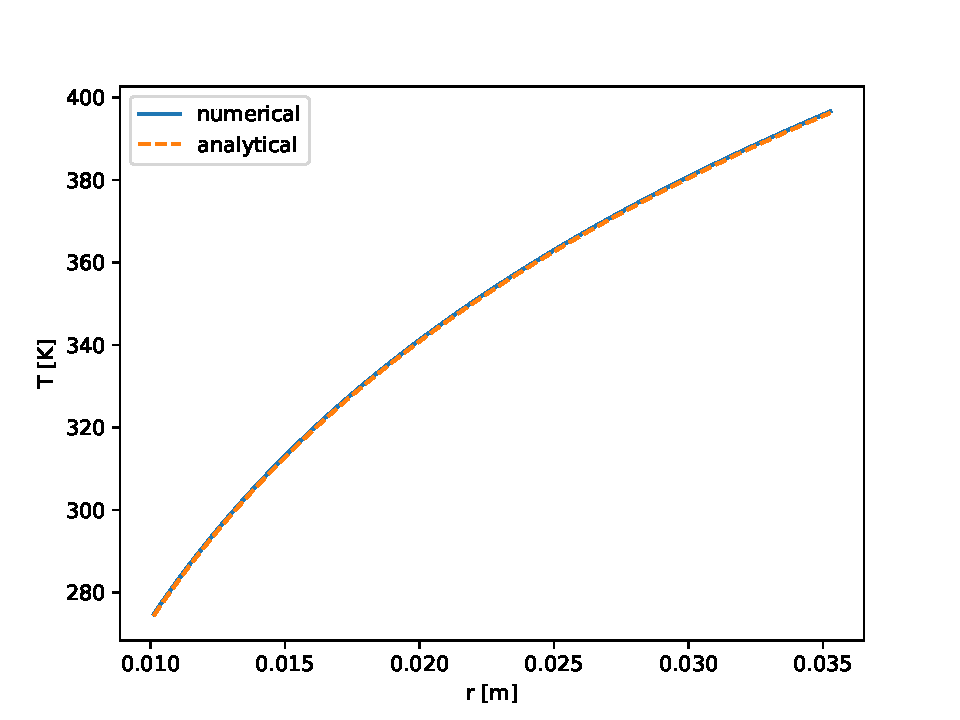
\includegraphics[width=\linewidth]{test_wall_conduction.pdf}
    \caption{Comparison of the analytical and numerical solution for the steady state heat conduction in a cylindrical shell.}
    \label{fig:validation_steady_state}
\end{figure}

\section{Dittus-Boelter}
The Dittus-Boelter correlation is a correlation intended for heat transfer from a smooth pipe to a turbulent single phase flow inside the pipe. The correlation for the Nusselt number is given by
\begin{equation}
    Nu = 0.023 Re^{0.8} Pr^{0.4}\;,
\end{equation} 
where the reynolds number is given by $Re = \frac{\rho_{\text{m}} u_{\text{m}} d}{\mu_{\text{m}}}$, where the subscript $m$ denotes the volume averaged quantity and $d$ is the diameter of the pipe. The Prandtl number is given by $Pr = \frac{C_{\text{p}} \mu_{\text{m}}}{k_{\text{m}}}$, where $C_{\text{p}}$ is the heat capacity at constant pressure, taking the mass average over the two phases. 
\section{Gungor-Winterton 87}
The gungor-winterton correlation is a correlation intended for flow boiling in a pipe, where the heat from the pipe wall causes the fluid to boil. The correlation is given in terms of an enhancement factor $E$, multiplied with the heat transfer predictet by the Dittus-Boelter correlation, if the pipe was filled with a single phase liquid
\begin{equation}
    h_{\ell} = Nu_{\ell} k_{\ell} / d = 0.023 \left(\frac{G  \left(1 - \beta_{\text{v}}\right) d}{\mu_{\ell}} \right)^{0.8} Pr^{0.4} k_{\ell} / d\;,
\end{equation}
where we have defined tha massflux $G = \sum_{k} \alpha_{k} \rho_{\text{k}} \left| u_{k}\right|$ and used the liquid prandtl number $Pr = \frac{C_{\text{p},\ell} \mu_{\ell}}{k_{\ell}}$. The enhancement factor is given by
\begin{equation}
    E = 1 + 3000Bo^{0.86} + 1.12 \left[\frac{\beta_{\text{v}}}{1-\beta_{\text{v}}}\right]^{0.75} \left[ \frac{\rho_{\ell}}{\rho_{\text{v}}} \right]^{0.41}\;.
\end{equation}
For a drift flux model, where the two phases move with different velocities, the mass fraction should be replaced with the flowing mass fraction
\begin{equation}
    \beta_{\text{v}}^{\text{flow}} = \frac{\alpha_{\text{v}} \rho_{\text{v}} \left| u_{\text{v}} \right|}{G}\;.
\end{equation}

\section{Pool boiling Rosenhow}
Eq 10.5 in fundamentals of heat and mass transfer by Incropera et al. gives the heat flux in pool boiling as
\begin{equation}
    q_{\text{s}}^{\prime\prime} = \mu_{\ell} h_{\text{v}\ell} \left[\frac{g\left( \rho_{\ell} - \rho_{\text{v}} \right)}{\sigma}\right]^{\frac{1}{2}} \left( \frac{c_{\text{p},\ell}\Delta T_{\text{e}}}{{C_{\text{s,f}}h_{\text{v}\ell}} Pr_{\ell}^n} \right)^{3}\;,
\end{equation}
where $\mu_{\ell}$ is the viscosity of the liquid phase, $h_{\text{v}\ell} = h_{\text{v}} - h_{\ell}$ is the latent heat of evaporation, $g$ is the gravitational constant, $\rho_{\ell}$ and $\rho_{\text{v}}$ are the densities of the liquid and vapor phase, $\sigma$ is the surface tension, $c_{\text{p},\ell}$ is the specific heat of the liquid phase, $\Delta T_{\text{e}} = T - T_{\text{s}}$ is the temperature difference between the wall $T_{\text{s}}$ and the fluid $T$ and $Pr_{\ell}$ is the Prandtl number of the liquid phsase. $C_{\text{s,f}}$ and $n$ are free empirical parameters related to the fluid-solid combination. Anders used $C_{\text{s,f}} = 0.013$ and $n=1.7$. 

This is the correlation used by Anders to calculate the heat transfer to the liquid phase. He needed to tweak $C_{\text{s,f}}$ to get the correct temperature in the wall. He seems to say that it does not describe the different experiments so well.
\section{Staggered solution strategy}
We solve the copuled fluid and wall heat transfer equations using a staggered solution strategy. In the calculation of the wall conduction, the fluid temperature is assumed to be constant. In the fluid calculation, the heat-flux from the solid is taken to be constant. Solving \cref{eq:heat_conduction} takes $T_{\text{fluid}}^n$ and $T_{\text{wall}}^n$ and returns $T_{wall}^{n+1}$ and $Q^{n+1}$. Similarly the fluid solver takes $Q^{n+1}$ as a constant while calculating $T_{\text{fluid}}^{n+1}$.

\end{document}